\documentclass[11pt]{article}
\usepackage[utf8]{inputenc}
\usepackage[english]{babel}
\usepackage{bilal2vec}

\title{SE 380 — Final Review}
\author{Bilal Khan\\
\href{mailto:bilal2vec@gmail.com}{bilal2vec@gmail.com}}
\date{\today}

\begin{document}

\maketitle

\tableofcontents

\section{Assignment 3}

\subsection{Question 1}

Consider the following model of a DC motor:

\[ G(s) = \dfrac{Y(s)}{U(s)} = \dfrac{K_m}{s(R_a (Js + b) + K_b K_m)} \]

where the value of all parameters is positive, the input $u(t) = \mathcal{L}^{-1}(U(s))$ is the voltage supplied to the motor, and the output $y(t) = \mathcal{L}^{-1}(Y(s))$ is the angle of the motor axle. Assume a unit step input voltage is supplied. 

\subsubsection{(a)} Find the transfer function betwen the angular speed - time derivative of the angle - and the input voltage.

\[ \omega(t) = y^\prime(t) \]
\[  G_\omega(s) = s G(s) = \dfrac{K_m}{R_a (Js + b) + K_b K_m} \]

\subsubsection{(b)} Find the steady-state angular speed of the motor axle

\begin{align*}
  \lim_{t \xrightarrow{} \infty} \omega(t) &= \lim_{s \xrightarrow{} 0} s G_\omega(s) U(s) \\
  &= \lim_{s \xrightarrow{} 0} s \dfrac{K_m}{R_a (Js + b) + K_b K_m} \dfrac{1}{s} \\
  &= \lim_{s \xrightarrow{} 0} \dfrac{K_m}{R_a (Js + b) + K_b K_m} = \dfrac{K_m}{R_a b + K_b K_m} \\
\end{align*}

\subsubsection{(c)} How long does the motor take to reach 99\% of its steady-state speed?

\begin{align*}
  G_\omega(s) &= \dfrac{K_m}{R_a (Js + b) + K_b K_m} \\
  &= \dfrac{K_m}{(R_a J) s + (R_a b + K_b K_m)} \\
  &= \dfrac{\frac{K_m}{R_a b + K_b K_m}}{\frac{R_a J}{R_a b + K_b K_m} s + 1} \\
\end{align*}

$\tau = \dfrac{R_a J}{R_a b + K_b K_m}$, we have that settling time @ 99\% is approximately $5 \tau = 5 \dfrac{R_a J}{R_a b + K_b K_m}$.

\subsection{Question 2}

Consider the following feedback control system.

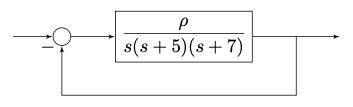
\includegraphics[width=200pt]{a3_q2.png}

Find the values of $\rho$ for which the closed-loop system is stable.

$L(s) = \dfrac{\rho}{s(s + 5)(s + 7)}$. We need to check if the poles of $1 + L(s)$ are in the left half of the plane.

\begin{align*}
  0 &= 1 + L(s) = 1 + \dfrac{\rho}{s(s^2 + 12s + 35)} \\
  &= 1 + \dfrac{\rho}{s^3 + 12s^2 + 35s} \\
  0 &= s^3 + 12s + 35s + \rho \\
\end{align*}

None of the given coefficients are negative, so we don't know if it is Hurwitz or not, all we can know is that for the system to be stable, $\rho > 0$.

\begin{table}[h]
  \centering
  \begin{tabular}{|c|c|c|}
  \hline
  $s^3$ & 1 & 35 \\
  $s^2$ & 12 & $\rho$ \\
  $s^1$ & $\frac{\rho - 12 \times 35}{-12}$ & 0 \\
  $s^0$ & $\rho$ & 0 \\
  \hline
  \end{tabular}
\end{table}

For all elements in the first column to be positive $\rho > 0$ and $\frac{\rho - 12 \times 35}{-12} > 0$.

\begin{align*}
  \frac{\rho - 12 \times 35}{-12} &> 0 \\
  \rho - 420 &< 0 \\
  \rho &< 420 \\
\end{align*}

The system is stable for $0 < \rho < 420$.

\subsection{Question 3}

Consider the following feedback control system.

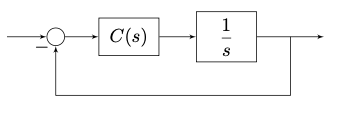
\includegraphics[width=200pt]{a3_q3.png}

Design a proportional controller a controller iwth transfer function $C(s) = K$ for some $K \in \mathbb{R}$ so that the closed-loop system satisfies the following specifications: It is stable, the steady state gain is $1$, and the settling time is less than $100ms$.

$L(s) = \dfrac{K}{s}$

$T(s) = \dfrac{L(s)}{1 + L(s)} = \dfrac{\frac{K}{s}}{1 + \frac{K}{s}} = \dfrac{K}{s + K}$

For the system to be stable, its poles are negative and so $K > 0$.

The steady-state gain is given by $\lim_{s \xrightarrow{} 0} s T(s) U(s) = \lim_{s \xrightarrow{} 0} \dfrac{K}{s + K} = \dfrac{K}{K} = 1$. So the steady-state gain is $1$. 

The settling time to 99\% is given by $5 \tau = 5 \dfrac{1}{K} < 0.1$. so $K > 50$.

This means that $C(s) = K$ for any $K > 50$

\section{Assignment 4}

\subsection{Question 1}

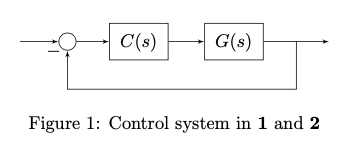
\includegraphics[width=200pt]{a4_1.png}

Consider the feedback control system where

\[ G(s) = \dfrac{5}{(1 + s) \left(1 + \dfrac{2 \zeta}{\omega_n} s + \dfrac{s^2}{\omega_n^2} \right)} \]

With $\omega_n = 10$ and $\zeta = 0.1$.

Design a controller $C(s)$ such that the closed-loop system has the following specifications: The steady state error in response to a unit step function is $e_\infty \leq 0.05$, the gain margin $k_m \geq 10$dB, and the phase margin $\phi_m \geq 60^\circ$.

We will design a controller with two parts: $C_1(s) = \mu / s^p$, to satisfy the steady state error requirement and we choose $p = 0$, and $C_2(s)$, to be a realizable controller that does not change the steady state behavior of the closed loop system to satisfy the gain and phase margin requirements.

\begin{align*}  
  y_\infty &= \dfrac{C_1(0)C_2(0)G(0)}{1 + C_1(0) C_2(0) C_3(0)} \\
  &= \dfrac{\mu * 1 * 5}{1 + \mu * 1 * 5} \\
  &= \dfrac{5 \mu}{1 + 5 \mu} \\
\end{align*}

For our steady state error requirement, we need $y_\infty \leq 0.05$, so manipulating this, we can see that we need $\mu \geq 3.8$. For simplicity, we choose $\mu = 4$.

For $C_2(s)$ to not change the steady state behavior of the closed loop system, we need $C_2(0) = 1$. We also need $C_2(s)$ to be realizable, so we choose to define it in the form $C_2(s) = \frac{L^\star(s)}{C_1(s) G(s)}$. The steady state gain of $G(s)$ is $5$, so we need $L^\star(0) = 5$. For the controller to be realizable, it must have the same degree as $G(s)$, 3. For a phase margin of at least $60^\circ$ and a gain margin of atleast $10$ dB, we will choose an arbitrary crossover point $\omega_c$ for the magnitude path of the bode plot of the controller to hit zero such that these two requirements are satisfied. We will choose $\omega_c = 10^1$ for simplicity (Any choice of $\omega_c$ will work). For the margins to be appropriately large, it is safe to place one pole at least one decade before $\omega_c$ and the other two poles at least one decade after $\omega_c$. 

\begin{align*}
  C_2(s) &= \dfrac{L^\star(s)}{C_1(s) G(s)} \\
  L^\star(s) &= \dfrac{5}{(1 + \frac{s}{10^0})(1 + \frac{s}{10^2})^2} \\
  C(s) &= C_1(s) C_2(s) \\
  &= C_1(s) L^\star(s) \dfrac{1}{G(s)} \\
  &= 4.0 \dfrac{5}{(1 + \frac{s}{10^0})(1 + \frac{s}{10^2})^2} \dfrac{(1 + s) \left(1 + \dfrac{2 \zeta}{\omega_n} s + \dfrac{s^2}{\omega_n^2} \right)}{5} \\
  &= 4.0 \cdot \dfrac{(1 + s) \left(1 + \dfrac{2 \zeta}{\omega_n} s + \dfrac{s^2}{\omega_n^2} \right)}{(1 + \frac{s}{10^0})(1 + \frac{s}{10^2})^2} \\
\end{align*}

In code, we can verify that the controller satisfies the requirements:

\inputminted{python}{a4_1.py}

$G(s)$ Bode Plot

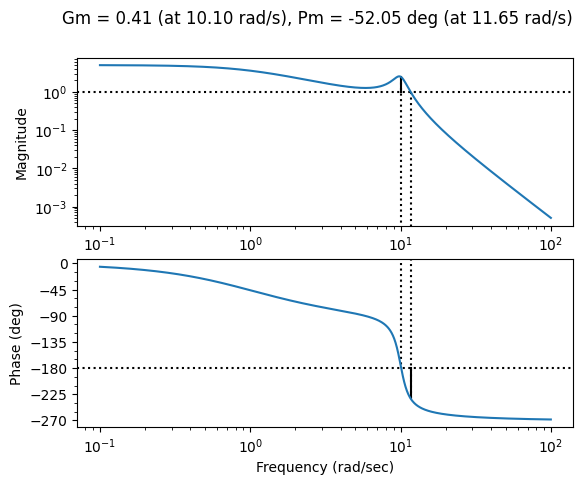
\includegraphics[width=200pt]{a4_2.png}
  
$G(s)$ Step Response

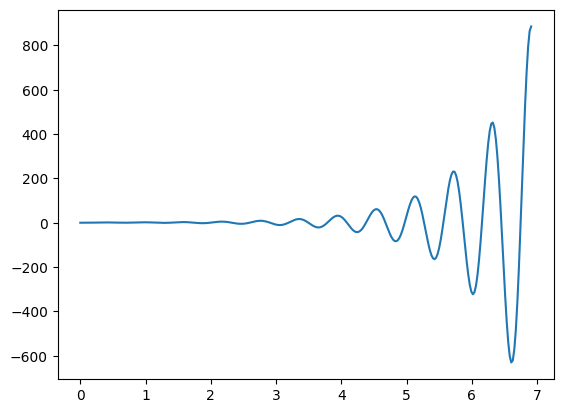
\includegraphics[width=200pt]{a4_3.png}

$C(s)$ Bode Plot

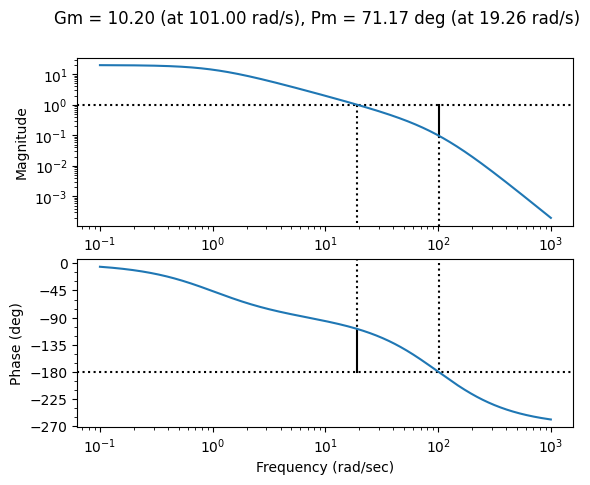
\includegraphics[width=200pt]{a4_4.png}
  
$C(s)$ Step Response

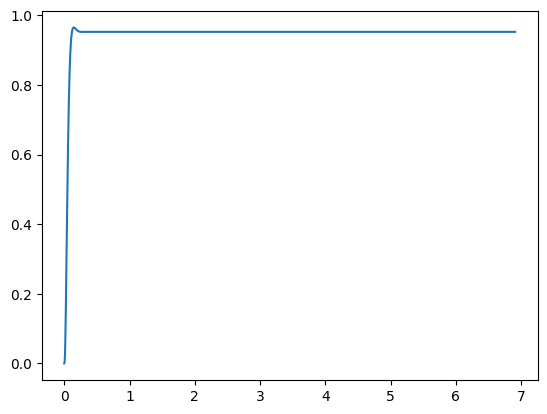
\includegraphics[width=200pt]{a4_5.png}

As we can see, the steady state error is less than $0.05$ (the output is $> 0.95$ at the end of the step response once the oscillations have settled), the gain margin is greater than $10$ dB, and the phase margin is greater than $60^\circ$.

\subsection{Question 2}

For the same feedback control system as part 1, design a controller $C(s)$ such athat the closed-loop system has the following specifications: No overshoot, the settling time at $1\%$ is $T_s^{1\%} \leq 0.5\%$, and the steady-state error in response to a unit step function is $|e_\infty| = 0$.

To do this we will adapt the controller from part 1. The controller from part one consists of $C_1(s)$ which was used to control the steady-state error, and $C_2(s)$ which was used to make the system stable and satisfy the gain and phase margin requirements. We will keep $C_2(s)$ the same since we still want the controller to stabilize the system (satisfying the gain and phase margin requirements is an extra bonus to keep the system in a "safe" region of stability) and replace $C_1(s)$ with a controller that will make the system have no overshoot and a settling time of $0.5\%$. To do this we want to use a proportional-integral controller as it increases the steady state gain to zero error and only marginally reduces the phase margin.

\[ mu = 2 \cdot \alpha \]
\[ c = \dfrac{\mu}{\alpha} \]
\[ T = \dfrac{10}{\omega_c} \]
\[ C_3(s) = c + \dfrac{c}{T} \dfrac{1}{s} \]

We will keep $\alpha = 10$ and $T = 10 / \omega_c$ using our crossover $\omega_c$ value from part 1 to keep the phase margin decline limited to $\approx 6\%$. We decide to set our increase of the steady state gain to $\mu = 2 \cdot \alpha$ instead of $\alpha$ since the value reached the settling time requirement too slowly.

We can verify that the controller satisfies the requirements in code:

\inputminted{python}{a4_2.py}

As we can see the overshoot is zero (modulo floating point rounding issues at $\approx 1e-8$), the error after $t = 0.5$ stays at less that $0.1\%$ satisfying the settling time requirement, and the steady state error is zero (neglibly small at $\approx 1e-8$).

$G(s)$ Bode Plot

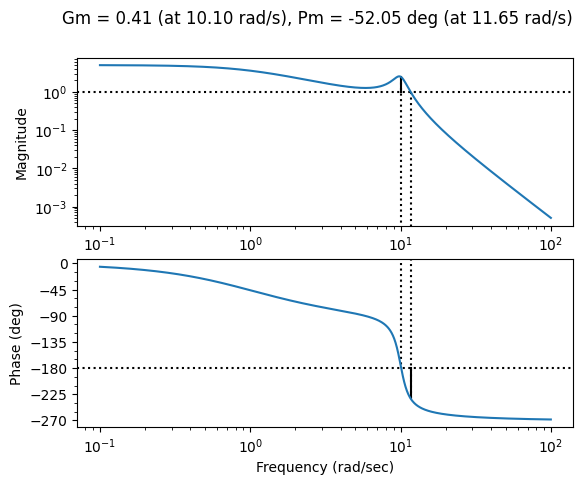
\includegraphics[width=200pt]{a4_6.png}
  
$G(s)$ Step Response

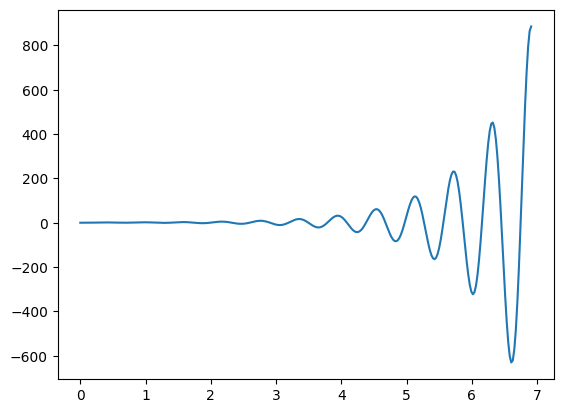
\includegraphics[width=200pt]{a4_7.png}

$C(s)$ Bode Plot

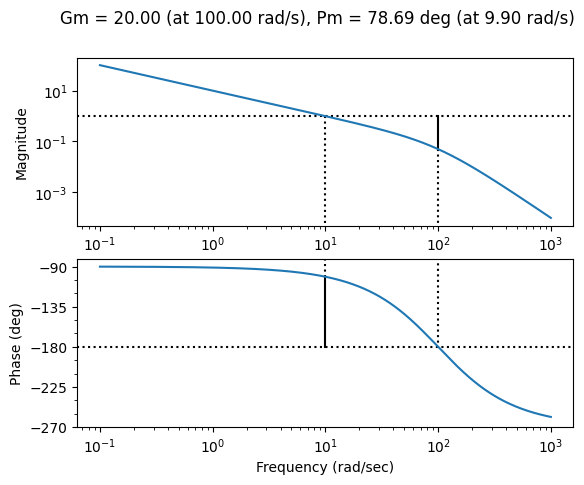
\includegraphics[width=200pt]{a4_8.png}
  
$C(s)$ Step Response

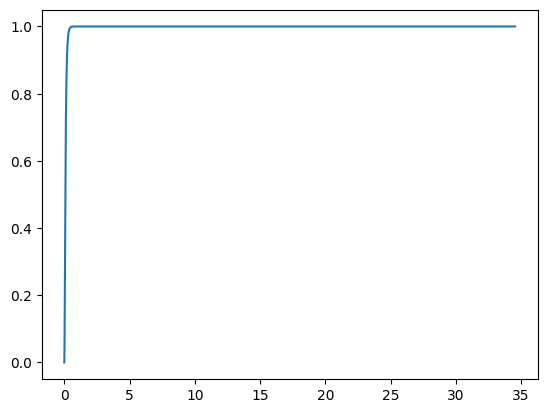
\includegraphics[width=200pt]{a4_9.png}

\section{Assignment 5}

\subsection{Question 1}

Design a lead-lag compensator $C(s)$ to control the system

\[ G(s) = \dfrac{1}{(1 + s)^3} \]


such that $L(s) = C(s)G(s)$ has steady-state gain greater than 100, crossover frequency greater than 5, and phase margin greater than $60^\circ$.

We will design a controller with two parts $C_1(s) = \dfrac{1}{(1 + s/p_1)(1 + s/p_2)^3}$ where $p_1, p_2$ are pole locations. This part is used to set the crossover frequency and make the controller realizable by increasing the degree of the denominator. We arbitrarily choose $\omega_c = 10$ as our crossover frequency and place poles one decade before and one decade after it. Note that the phase margin should be $90^\circ$ as the pole one decade before the crossover frequency will contribute a phase of $-90^\circ$ to the bode plot. We place three poles one decade after the crossover frequency to ensure that our final controller will be realizable.

\[ C_1(s) = \dfrac{1}{(1 + (s / 1)) (1 + (s / 100)^3)} \]

To satisfy the steady state gain requirement, we need $F(0) \geq 100$ and so we choose a steady state gain of $101$. We use a phase-lag controller to improve static performance withouth losing stability: $C_2(s) = \mu \frac{1 + T s}{1 + \alpha T s}$. We choose the default value of $\alpha = 10$ and $T = 10 / \omega_c$ to limit the phase margin decrease at the crossover frequency to $\approx 6\%$, which gives us more than enough phase margin to satisfy the requirement. We choose $\mu = 101$ since we know that phase-lag controllers increase the steady state gain at low frequencies (and by extension the steady-state gain) by a factor of $\mu$.

\[ C_2(s) = 101 \dfrac{1 + s}{1 + 10s} \]

We then combine the two controllers and cancel out the $G(s)$ to get our final controller. Note that the controller is proper.

\[ C(s) = C_1(s) C_2(s) / G(s) = 101 \dfrac{1}{(1 + (s / 1)) (1 + (s / 100)^3)} \dfrac{1 + s}{1 + 10s} \dfrac{(1 + s)^3}{1} \]

In code:

\begin{minted}{python}
import math
import numpy as np
import control as ct
import matplotlib.pyplot as plt

s = ct.tf('s')
G = 1 / (1 + s)**3

plt.figure()
ct.bode_plot(G, margins=True)
plt.show()

plt.figure()
t, y = ct.step_response(G)
plt.plot(t, y)
plt.show()

omega_c = 10

pole_1 = omega_c / 10
pole_2 = omega_c / 0.1
C_1 = 1 / ((1 + (s / pole_1)) * (1 + (s / pole_2)) ** 3)

alpha_2 = 10
mu_2 = 101
T_2 = 10 / omega_c
C_2 = mu_2 * (1 + T_2 * s) / (1 + alpha_2 * T_2 * s)

C = C_1 * C_2 * (1 / G)

plt.figure()
ct.bode_plot(C * G, margins=True)
plt.show()

plt.figure()
t, y = ct.step_response(C * G)
plt.plot(t, y)
plt.show()
\end{minted}

$G(s)$ bode plot

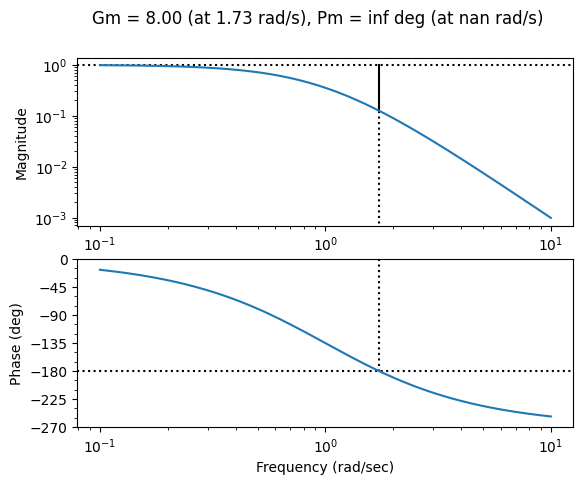
\includegraphics[width=300pt]{a5_1.png}

$G(s)$ step response

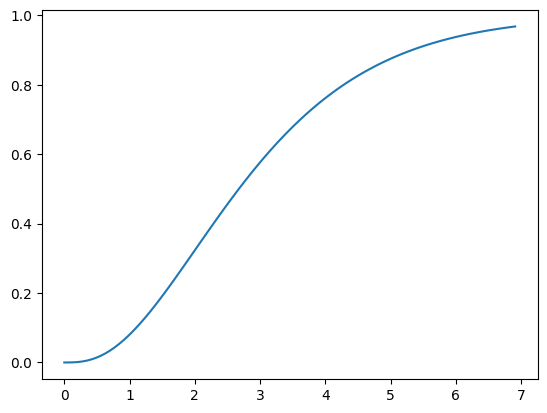
\includegraphics[width=300pt]{a5_2.png}

$C(s)$ bode plot

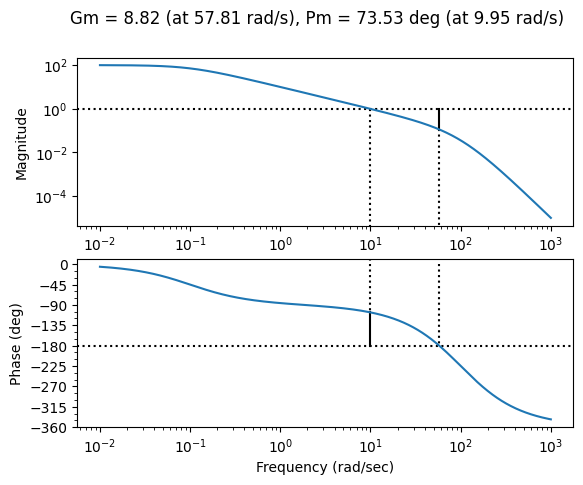
\includegraphics[width=300pt]{a5_3.png}

$C(s)$ step response

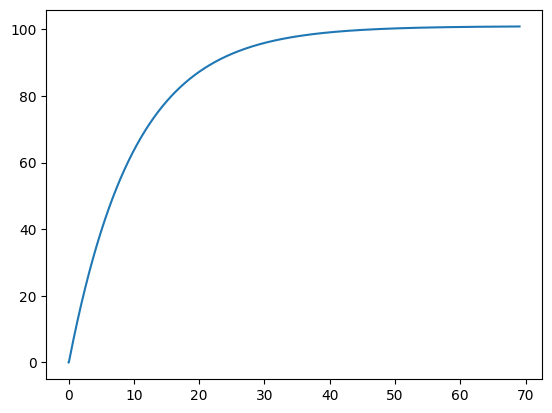
\includegraphics[width=300pt]{a5_4.png}

\subsection{Question 2}

Design a proportional controller for the system $G(s) = \frac{100(s + 1)}{(s - 1)(s^2 + 5s + 10)}$ such that the closed-loop system is stble and the damping of the complex-conjugate poles is greater than $0.45$. Note from the textbook that the phase margin of a second order system is approximately equal to 100 times the damping of the poles as long as the phase margin in between 0 and 60 degrees. A proportional controller is of the form $C(s) = k_p$. Through trial and error we find that $k_p = 0.2$ satisfies the phase margin requirements.

In code:

\begin{minted}{python}
import math
import numpy as np
import control as ct
import matplotlib.pyplot as plt

s = ct.tf('s')
G = (100 * (s + 1)) / ((s - 1) * (s**2 + 5 * s + 10))

plt.figure()
ct.bode_plot(G, margins=True)
plt.show()

plt.figure()
t, y = ct.step_response(G / (1 + G))
plt.plot(t, y)
plt.show()

s = ct.tf('s')
G = (100 * (s + 1)) / ((s - 1) * (s**2 + 5 * s + 10))

plt.figure()
ct.bode_plot(0.2 * G, margins=True)
plt.show()

plt.figure()
t, y = ct.step_response(G / (1 + G))
plt.plot(t, y)
plt.show()
\end{minted}

$G(s)$ bode plot

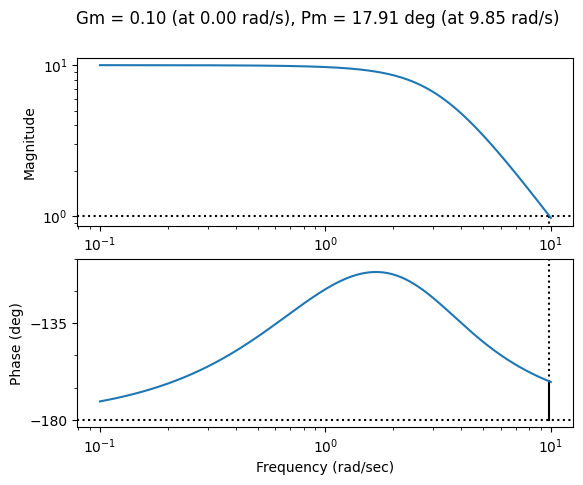
\includegraphics[width=300pt]{a5_5.png}

$G(s)$ step response

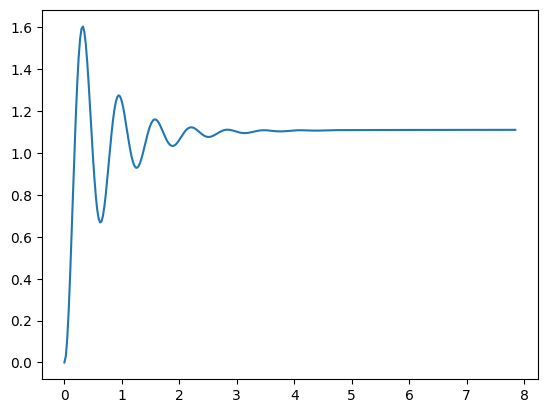
\includegraphics[width=300pt]{a5_6.png}

$C(s)$ bode plot

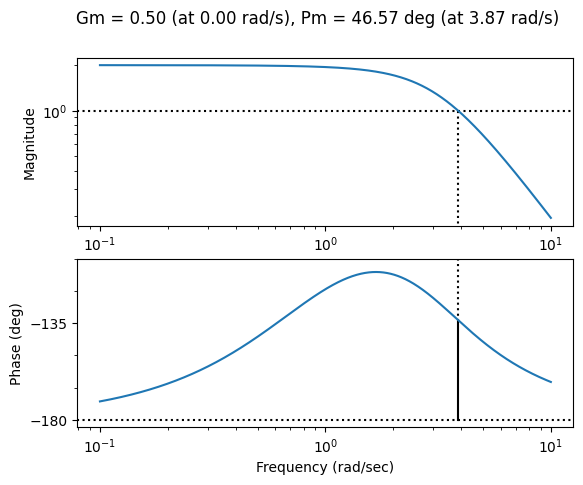
\includegraphics[width=300pt]{a5_7.png}

$C(s)$ step response

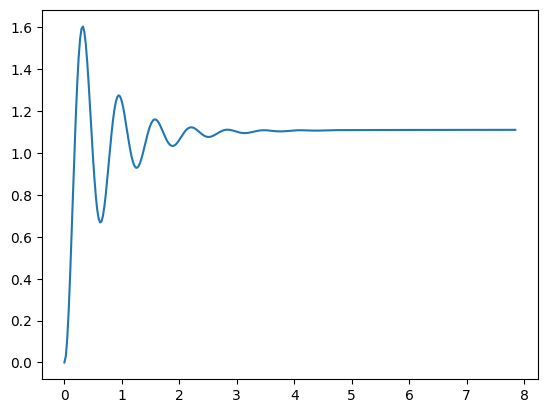
\includegraphics[width=300pt]{a5_8.png}

\section{E6.1}

A system has a characteristic equation $s^3 + Ks^2 + (1 + K)s + 6 = 0$. Determine the range of $K$ for a stable system

Answer: $K > 2$

\begin{table}[h]
  \centering
  \begin{tabular}{|c|c|c|}
  \hline
  $s^3$ & 1 & 1 + K \\
  $s^2$ & K & 6 \\
  $s^1$ & $- (1/K) (1(6) - K (1 + K))$ & $- (1 / K) (1(0) - 0(K)) = 0$ \\
  \hline
  \end{tabular}
\end{table}

\begin{align*}
  \dfrac{-1}{K} (6 - K - K^2) > 0 \\
  K^2 + K - 6 > 0 \\
  (K + 3)(K - 2) > 0 \\  
\end{align*}

Gives us conditions $K > -3, K > 2$ and so $K > 2$.


\section{E6.12}

A system has the second-order characteristic equation $s^2 + as + b = 0$, where $a, b$ are constant parameters. Determine the necessary and sufficient conditions for the system to be stable. Is it possible to determine stability of a second-order system just by inspecting the coefficients of the characteristic equation?.

Yes, the roots need to have real negative parts

\section{E6.13}

Consider the feedback system below. Determine the range of $K_p$ and $K_D$ for the stability of the closed-loop system.

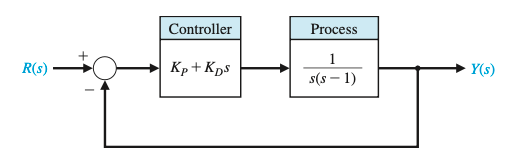
\includegraphics[width=300pt]{e6.13.png}

The overall transfer function of the system is given as $L(s) / (1 + L(s))$ where $L(s) = \dfrac{K_p + K_d s}{s(s - 1)}$. We need the real parts of the roots of $1 + L(s)$ to be negative for the system to be stable. The roots of $1 + L(s)$ are given by the roots of $s^2 - s + K_p + K_d s = 0$ which can be solved for using the quadratic formula.

\section{E6.14}

By using magnetic bearings, a rotor is supported contactless. The technique of contactless support for rotors becomes mroe important in light and heavy industrial applications. The matrix differential equation fro a magnetic bearing is

\[
  \dot{x(t)} = \begin{bmatrix}
    0 & 1 & 0 \\
    -3 & -1 & 0 \\
    -2 & -1 & -2 \\
  \end{bmatrix}
  x(t)
\]

where $x^T(t) = (y(t), \dot{y(t)}, i(t))$, $y(t)$ being the bearing gap, and $i(t)$ being the electromagnetic current. Determine whether the system is stable.

Answer: The system is stable

Find the characteristic polynomial of the system using $\det(A - \lambda I)$ and solve this for $\lambda$ to find the eigenvalues of the system. The system is stable if the real parts of the eigenvalues are negative. This is a 3x3 matrix so lol I'm not doing this by hand.

\section{E6.24}

Consider the system represented in state variable form

\begin{align*}
  \dot{x(t)} &= Ax(t) + Bu(t) \\
  y(t) &= Cx(t) + Du(t) \\
\end{align*}

where

\[
  A = \begin{bmatrix}
    0 & 1 & 0 \\
    0 & 0 & 1 \\
    -k & -k & -k \\
  \end{bmatrix}
  ,
  B = \begin{bmatrix}
    0 \\
    0 \\
    1 \\
  \end{bmatrix}
  ,
  C = \begin{bmatrix}
    1 & 0 & 0 \\
  \end{bmatrix}
  ,
  D = \begin{bmatrix}
    0 \\
  \end{bmatrix}
\]

What is the system transfer function and for what values of $k$ is the system stable.

Compute the transfer function using $G(s) = C (sI - A)^{-1} B + D$, then check if the system is stable by checking if the real parts of the poles of the transfer function are negative. 3x3 matrix, not doing by hand.

\section{E6.25}

A closed-loop feedback system is shown in the figure below. For what range of values of the parameters $K, p$ is the system stable?

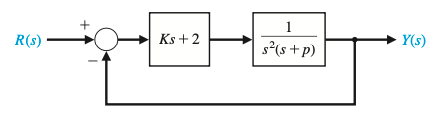
\includegraphics[width=300pt]{e6.25.png}

The overall transfer function of the system is given as $L(s) / (1 + L(s))$ where $L(s) = \dfrac{Ks + 2}{s^2(s + p)}$. We need the real parts of the roots of $1 + L(s)$ to be negative for the system to be stable.

\begin{align*}
  1 + L(s) &= 0 = 1 + \dfrac{Ks + 2}{s^2(s + p)} \\
  1 + \dfrac{Ks + 2}{s^2(s + p)} &= 0 \\
  s^2(s + p) + Ks + 2 &= 0 \\
  s^3 + ps^2 + Ks + 2 &= 0 \\
\end{align*}

Solve this using a Routh Table

\begin{table}[h]
  \centering
  \begin{tabular}{|c|c|c|}
  \hline
  $s^3$ & 1 & K \\
  $s^2$ & p & 2 \\
  $s^1$ & $-(1/p) (1(2) - K(p))$ & 0 \\
  \hline
  \end{tabular}
\end{table}

\begin{align*}
  \dfrac{-1}{p} (2 - Kp) &> 0 \\
  2 - Kp &< 0 \\
  Kp &> 2 \\
  K &> \dfrac{2}{p} \\
  p &> 0 \\
\end{align*}

\section{E7.1}

Consider a device that consists of a ball rolling on the inside rim of a hoop. This omdel is similar to the problem of liquid fuel sloshing in a rocket. The hoop is free to rotate about its horizontal principle axis. The angular position of the hoop may be controlled via the torque $T(\tau)$ applied to the hoop from a torque motor attached to the hoop drive shaft. If negative feedback is used, the system characterisitic equation is $1 + \frac{Ks(s + 4)}{s^2 + 2s + 2} = 0$. Sketch the root locus, find the gain when the roots are both equal, find these two equal roots, and find the settling time of the system when the roots are equal.

The system characteristic equation can be rearranged to:

\begin{align*}
  s^2 + 2s + 2 + Ks(s + 4) = 0 \\
  s^2 + 2s + 2 + Ks^2 + 4Ks = 0 \\
  (1 + K)s^2 + (2 + 4K)s + 2 = 0 \\
\end{align*}

Find the roots of this equation using the quadratic formula to find the two roots of the system. Draw the root locus by *skipping*. I'm not sure how to find the gain?!?. The settling time can be found by finding the roots of this quadratic for some $K$ and reading them out in the form $\zeta \omega_n \pm j \sqrt{1 - \zeta^2} \omega_n$. Settling time is approximately $4 / \zeta \omega_n$.

\section{E7.2}

A tape recorder with a unity feedback speed controller has teh loop transfer function $L(s) = G_c(s) G(s) = \dfrac{K}{s(s+ 2)(s^2 + 4s + 5)}$ Sketch a root locus for $K$ and show that the dominant roots are $s = -0.35 \pm j 0.80$ when $K = 6.5$, then calculate the settling time and overshoot for a step input.

Not sketching root locus. The dominant poles in this TF are the ones for the $s^2 + 4s + 5$ term, use this to find the values of $\zeta, \omega_n$ and then use these to find the settling time and overshoot.

\section{E7.3}

A unity feedback control system for an automobile suspension tester has the loop transfer function $L(s) = G_c(s) G(s) = \dfrac{K(s^2 + 4s + 8)}{s^2(s + 4)}$. We desire the dominant roots to have a $\zeta = 0.5$. Using the root locus, show that $K = 7.35$ is required and the dominant roots are $s = -1.3 \pm j 2.2$.

Not sketching root locus. The characteristic equation of the system is $s^2 (s + 4) + K(s^2 + 4s + 8) = 0$. The dominant poles are the ones for the $s^2 + 4s + 8$ term, use this to find the values of $\zeta, \omega_n$ and then use these to show that the values match the given values.

\section{E7.8}

Sketch the root locus for a unity feedback system with $L(s) = G_c(s) G(s) = \dfrac{K(s + 1)}{s^2 (s + 9)}$. Find the gain and roots when all three roots are real and equal.

Not sketching root locus. The characteristic equation of the system is $s^2 (s + 9) + K(s + 1) = 0$. Equate the coefficients of the characteristic equation to that of $(s - \lambda)^3$ to find the roots when all three roots are real and equal. The value for the gain $K$ can be found when equating the coefficients of both representations of the characteristic equation.

\section{E7.20}

A unity feedback system has a loop transfer function $L(s) = G_c(s) G(s) = \dfrac{K(s + 1)}{s(s - 2)(s + 6)}$. Determine the range of $K$ for stability, sketch the root locus, and determine the maximum $\zeta$ of the stable complex roots. 

Answer: $K > 16$, $\zeta = 0.25$.

Not finding root locus. Characteristic equation given by $s(s - 2)(s + 6) + K(s + 1) = 0$. Use a Routh table to find the bounds on stable values for $K$ and use it to find the maximum $\zeta$ of the stable complex roots.

\section{E10.1}

A negative feedback control system has a transfer function $G(s) = \dfrac{K}{s + 2}$. We select a compensator $G_c(s) = \dfrac{s + a}{s}$ in order to acheive zero steady-state error for a step input. Select a and K so that the percent the overshoot to a step is $\leq 5\%$ and settling time (with a 2\% criterion) is $\leq 1s$.

Answer: $K = 6, a = 5.6$.

Use the overshoot equation to find a value for $\zeta$, and then use the settling time equation to find a value for $\omega_n$ using the $1 = 4 / \zeta \omega_n$ equation. The dominant poles are then located at $\zeta \omega_n \pm j \sqrt{1 - \zeta^2} \omega_n$. 

Now we want to choose $a$ and $K$ so that the overall system has poles at this location. Is there's any way to do this without using python?

\section{E10.2}

A control system with negative unity feedback has a process $G(s) = \dfrac{400}{s(s + 40)}$, and we select a proportional plus integral compensator where $G_c(s) = K_p + \dfrac{K_I}{s}$. Note that the steady-state error of this system for a ramp input is zero. Set $K_I = 1$ and find a suitable value of $K_P$ so the step response will have a percent overshoot $\leq 20\%$. What is the expected settling time (with a 2\% criterion) of the compensated system?

Answer: $K_P = 0.5$.

Same process of finding $\zeta, \omega_n$ to find the dominant poles, then find $K_P$ so that the system has poles at this location. Doable without python?

\section{E10.3}

A unity feedback control system in a manufacturing system has a process transfer function $G(s) = \dfrac{e^{-s}}{s + 1}$. And it is proposed to use a compensator to acheive a percent overshoot $\leq 5\%$ to a step input. The compensator is $G_c(s) = K \left(1 + \dfrac{1}{\tau s} \right)$ which proveides proportional plus integral control. Show one solution is $K = 0.5, \tau = 1$.

Same as before??

\section{E11.1}

The ability to balance actively is a key ingredient in the mobility of a device that hops and runs on one springy leg. The control of the attitude of the device uses a gyroscope and a feedback such that $u(t) = Kx(t)$, where $K = \begin{bmatrix} -k & 0 \\ 0 & -2k \\ \end{bmatrix}$ and $\dot{x(t)} = A x(t) + B u(t)$, where $A = \begin{bmatrix} 0 & 1 \\ -1 & 0 \\ \end{bmatrix}$ and $B = I$. Determine a value of $K$ so that the response of each hop is critically damped.

Too complicated, not doing.

\section{E11.2}

A magnetically suspended steel ball can be described by the linear equation 

\[ \dot{x(t)} = \begin{bmatrix} 0 & 1 \\ 9 & 0 \\ \end{bmatrix} x(t) + \begin{bmatrix} 0 \\ 1 \\ \end{bmatrix} u(t) \]

The state variables are $x_1(t)$ being position and $x_2(t)$ being velocity, and both are measurable. Select a feedback so that the system is critically damped and the settling time with a 2\% criterion is $4s$. Choose the feedback in the form

\[ u(t) = -k_1 x_1(t) - k_2 x_2(t) + r(t) \]

where $r(t)$ is the reference input and the gains $k_1, k_2$ are to be determined.

Critically damped means $\zeta = 1$, 2\% settling time at 4s with $zeta = 1$ works out nicely to have $\omega_n = 1$. The characteristic equation is then just $s^2 + 2s + 1 = 0$ and so the two poles are at $s = -1$. Manually compute the characteristic equation of the system $|\lambda I - (A - BK)|$ to find the the roots of the system. Then equate the coefficients of the characteristic equation with our placed poles to find the values of $k_1, k_2$.

\section{P11.22}

A manipulator control system has a loop transfer function of $G(s) = \dfrac{1}{s(s + 0.4)}$ and negative unity feedback. Represent this system by a state variable signal-flow graph or block diagram and a vector differential equation. Plot the response of the closed-loop system to a step input, use state variable feedback so that the percent overshoot is $5\%$ and and the settling time (with a $2\%$ criterion) is $1.35s$. Plot the response of the state variable feedback system to a step input.

Too long, not doing but same general idea.

\section{P11.28.}

Consider the single-input, single-output system described by 

\begin{align*}
  \dot{x(t)} &= A x(t) + B u(t) \\
  y(t) &= C x(t) \\
  A &= \begin{bmatrix}
    0 & 1 \\
    -16 & -8 \\
  \end{bmatrix} \\
  B &= \begin{bmatrix}
    0 \\
    K \\
  \end{bmatrix} \\
  C &= \begin{bmatrix}
    1 & 0 \\
  \end{bmatrix} \\
\end{align*}

Determine the value of $K$ resulting in a zero steady-state tracking error when $u(t)$ is a unity step function for $t \geq 0$. The tracking error is defined as $e(t) = u(t) - y(t)$. Plot the response of the system to a unit step input and verify that the tracking error is zero.

Not doing.

\end{document}
